% Created 2017-03-12 Sun 14:54
% Intended LaTeX compiler: pdflatex
\documentclass[a4paper,11pt]{article}
\usepackage[utf8]{inputenc}
\usepackage[T1]{fontenc}
\usepackage{graphicx}
\usepackage{grffile}
\usepackage{longtable}
\usepackage{wrapfig}
\usepackage{rotating}
\usepackage[normalem]{ulem}
\usepackage{amsmath}
\usepackage{textcomp}
\usepackage{amssymb}
\usepackage{capt-of}
\usepackage{hyperref}
\usepackage[margin=1in]{geometry}
\usepackage{setspace}
\onehalfspacing
\usepackage{parskip}
\usepackage{amsthm}
\usepackage{amsmath}
\usepackage{mathtools}
\usepackage{hyperref}
\usepackage{graphicx}
\usepackage{tabularx}
\usepackage{booktabs}
\hypersetup{colorlinks,citecolor=black,filecolor=black,linkcolor=black,urlcolor=black}
\newtheorem{definition}{Definition}
\newtheorem{theorem}{Theorem}
\newcommand{\rarrowd}[1]{\xrightarrow{\text{ \textit #1 }}}
\DeclareMathOperator*{\plim}{plim}
\newcommand{\plimn}{\plim_{n \rightarrow \infty}}
\setcounter{secnumdepth}{2}
\author{Zheng Tian}
\date{}
\title{Lecture 6: Linear Regression with One Regressor}
\hypersetup{
 pdfauthor={Zheng Tian},
 pdftitle={Lecture 6: Linear Regression with One Regressor},
 pdfkeywords={},
 pdfsubject={},
 pdfcreator={Emacs 25.1.1 (Org mode 9.0.3)},
 pdflang={English}}
\begin{document}

\maketitle
\setcounter{tocdepth}{1}
\tableofcontents



\section{Introduction}
\label{sec:orgacdae23}

This lecture introduces a linear regression model with one regressor
called a simple linear regression model. We will learn the ordinary
least squares (OLS) method to estimate a simple linear regression
model, discuss the algebraic and statistical properties of the OLS
estimator, introduce two measures of goodness of fit, and bring up three least
squares assumptions for a linear regression model. As an example, we
apply the OLS estimation method to a linear model of test scores and
class sizes in California school districts.

This lecture lays out foundations for all lectures to come. Although
in practice we seldom use a linear regression model with only one
regressor, the essential principles of the OLS estimation method and
hypothesis testing are the same for a linear regression model with
multiple regressors.


\section{The Linear Regression Model}
\label{sec:org04b5f32}

\subsection{What is regression?}
\label{sec:org96fcdd9}

\subsubsection*{Definition of \textbf{regress} in Merriam-Webster's dictionary}
\label{sec:org2c1c9ef}

Merriam-Webster gives the following definition of the word "regress":
\begin{enumerate}
\item An act or the privilege of going or coming back
\item Movement backward to a previous and especially worse or more
primitive state or condition
\item The act of reasoning backward
\end{enumerate}

\subsubsection*{The meaning of regression in statistics?}
\label{sec:org6a0dc35}

In statistical modeling, regression analysis is a statistical process
for estimating the relationships among variables.\footnote{Wikipedia, the free encyclopedia. Regression analysis. Retrieved from \url{https://en.wikipedia.org/wiki/Regression\_analysis}} Specifically,
most regression analysis focus on the conditional mean of the
dependent variable given the independent variables, which is a
function of the values of independent variables.

A very simple functional form of a conditional expectation is a linear
function. That is, we can model the conditional mean as follows,
\begin{equation}
\label{eq:genpopreg}
\mathrm{E}(Y \mid X = x) = f(x) = \beta_{0} + \beta_1 x
\end{equation}
Equation \ref{eq:genpopreg} is called a \textbf{simple linear regression
function}.


\subsection{An example: Test scores versus class size}
\label{sec:org3132d00}

Let's go back to the example of California school districts,
introduced in Lecture 1.

\subsubsection*{Research question:}
\label{sec:org880fd0c}

The research question of this application is: Can reducing class size
increase students' test scores?

\subsubsection*{How can we answer the question?}
\label{sec:org762280e}

\begin{itemize}
\item We randomly choose 42 students and divide them into two classes,
with one having 20 students and another having 22. And they are
taught with the same subject and by the same teachers.

\item Randomization ensures that it is the difference in class sizes of
the two classes that is the only factor affecting test scores.

\item After a test for both classes, we then compute the average test
scores that can be expressed as,
\begin{gather*}
\mathrm{E}(TestScore | ClassSize = 20) \\
\mathrm{E}(TestScore | ClassSize = 22)
\end{gather*}

\item Then the effect of class size on test scores is the difference in
the conditional means, i.e.,
\begin{equation*}
\mathrm{E}(TestScore | ClassSize = 20) - \mathrm{E}(TestScore | ClassSize = 22)
\end{equation*}

\item If the difference is large enough, we can say that reducing class
can improve students' test performance.
\end{itemize}

\subsubsection*{A simple linear regression model of test scores v.s. class size}
\label{sec:org7fa6bcf}

As mentioned above, a simple linear regression function can be used to
describe the relationship between test scores and class sizes. Since
it regards the association between these two variable for the whole
population, we call this regression function as the \textbf{population
regression function} or the \textbf{population regression line}, taking the
following form,
\begin{equation}
\label{eq:popreg-testscore}
\mathrm{E}(TestScore | ClassSzie) = \beta_0 + \beta_1 ClassSize
\end{equation}

By calculating the conditional expectation, some other factors, apart
from class sizes, are left out of the population regression
function. Although these factors may also influence test scores, they are
either unimportant in your reasoning or unable to be measured. We can
lump all these factors into a single term, and set up a \textbf{simple linear
regression model} as follows,
\begin{equation}
\label{eq:regmodel-testscore}
TestScore = \beta_0 + \beta_1 ClassSize + OtherFactors
\end{equation}

If we assume \(\mathrm{E}(OtherFactors | ClassSize) = 0\), then the
simple linear regression model (Eq. \ref{eq:regmodel-testscore})
becomes the population regression line
(Eq. \ref{eq:popreg-testscore}).

\subsubsection*{A distinction between the population regression function and the population regression model}
\label{sec:orge1a7a72}

Note that here we have two concepts: the population regression
function and the population regression model. What's their difference?
Simply put,
\begin{itemize}
\item A population regression function gives us a deterministic
relation between class size and the expectation of test scores. That
is, when we have a value of class size and know the values of
\(\beta_0\) and \(\beta_1\), there is one and only one
expected value of test scores associated with this class size.
However, we cannot compute the exact value of the test score of a
particular observation.
\item A population regression model, by including other factors, gives us
a complete description of a data generating process (DGP). That is,
when we have all the values of class sizes and other factors and
know \(\beta_0\) and \(\beta_1\), we can generate all the values of test
scores. Also, when we consider other factors as a random variable,
the association between test scores and class size is not
deterministic, depending on the value of other factors.
\end{itemize}

\subsubsection*{An interpretation of the population regression model}
\label{sec:org635c1c9}

Now we have set up the simple linear regression model,
\begin{equation*}
TestScore = \beta_0 + \beta_1 ClassSize + OtherFactors
\end{equation*}
What is \(\beta_1\) and \(\beta_0\) represent in the model?

\begin{itemize}
\item Interpret \(\beta_1\)
\label{sec:org66d7351}

Let's first look at \(\beta_1\). When we hold other factors constant,
the only reason for a change in test scores is a change in class
size. Denote \(\Delta TestScore\) and \(\Delta ClassSize\) to
be their respective change. According to the above regression model,
holding other factors constant, we have
\[ \Delta TestScore = \beta_1 \Delta ClassSize  \]
where \(\beta_0\) is removed because it is also a constant. Then, we get
\[ \beta_1 = \frac{\Delta TestScore}{\Delta ClassSize} \]
That is, \(\beta_1\) measures the change in the test score resulting
from a \textbf{one-unit change} in the class size. When \(TestScore\) and
\(ClassSize\) are two continuous variable, we can write \(\beta_1\) as
\[\beta_1 = \frac{\mathrm{d} TestScore}{\mathrm{d} ClassSize}  \]
Hence, we often call \(\beta_1\) as the \textbf{marginal effect} of the class
size on the test score.

The phrase of "holding other factors constant" is important. Without
it, we cannot disentangle the effect of class sizes on test scores
from other factors. "Holding other things constant" is often expressed
as the notion of \textbf{ceteris paribus}.

\item Interpret \(\beta_0\)
\label{sec:orgf6f4f95}

\(\beta_0\) is the intercept in the model. Sometimes it bears real
meanings, but sometimes it merely presents as an intercept. In this
regression model, \(\beta_0\) is the test score when the class size and
other factors are all zero, which is obviously nonsensical. Thus,
\(\beta_0\) does not have a real meaning in this model, and it just
determines where the population regression line intersects the Y
axis.
\end{itemize}


\subsection{The general linear regression model}
\label{sec:orge54441d}

Let's generalize test scores and class sizes to be two random
variables \(Y\) and \(X\). For both, there are \(n\) observations so that
each observation \(i = 1, 2, 3, \ldots\) is associated with a pair of
values of \((X_i, Y_i)\).

Then a \textbf{simple linear regression model} that associates \(Y\) with \(X\) is
\begin{equation}
\label{eq:single-regress}
Y_i = \beta_0 + \beta_1 X_i + u_i, \text{ for } i = 1, \ldots, n
\end{equation}

\begin{itemize}
\item \(Y_i\) is called the dependent variable, the regressand, or the LHS
(left-hand side) variable.
\item \(X_i\) is called the independent variable, the regressor, or the RHS
(right-hand side) variable.
\item \(\beta_{0}\) is the intercept, or the constant term. It can either have
economic meaning or have merely mathematical sense, which determines
the level of the regression line, i.e., the point of intersection
with the Y axis.
\item \(\beta_{1}\) is the slope of the population regression line. Since
\(\beta_1 = \mathrm{d}Y_i/ \mathrm{d}X_i\), it is the marginal effect
of \(X\) on \(Y\). That is, holding other things constant, one unit
change in \(X\) will make \(Y\) change by \(\beta_1\) units.
\item \(u_i\) is the error term. \(u_i = Y_i - (\beta_0 + \beta_1 X_i)\)
incorporates all the other factors besides \(X\) that determine the
value of \(Y\).
\item \(\beta_{0} + \beta_{1}X_{i}\) represents the population regression
function(or the population regression line).
\end{itemize}


\subsection{An graphical illustration of a linear regression model}
\label{sec:org2472aaa}

The relationship between the data points, the population regression
line, and the errors (other factors) are illustrated in Figure \ref{fig:org355bbd5}.

\begin{figure}[htbp]
\centering
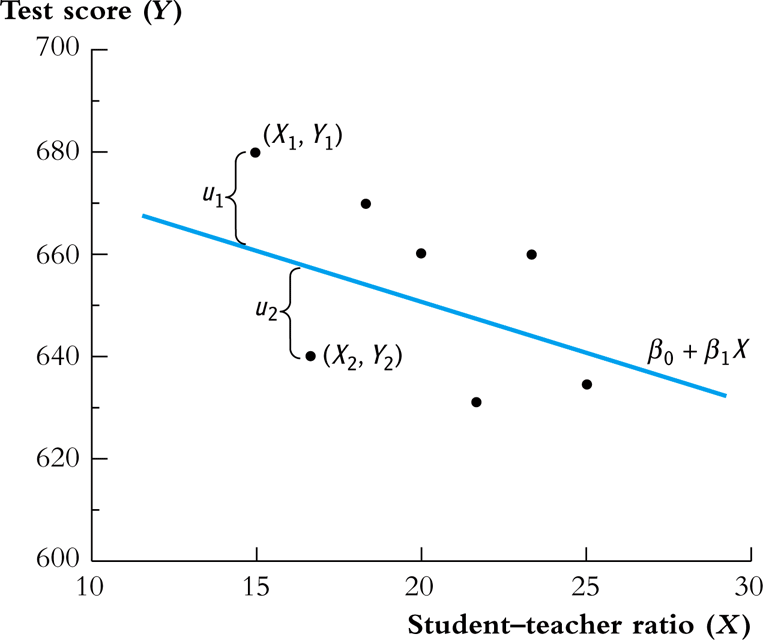
\includegraphics[width=0.75\textwidth]{figure/fig-4-1.png}
\caption{\label{fig:org355bbd5}
The Population Regression Line}
\end{figure}
\end{document}